Conclusa la presentazione delle scelte adottate in fase di impostazione delle sperimentazioni, 
si procede in questo capitolo con l'esposizione dei risultati ottenuti. 

Per effettuare la risoluzione delle diverse istanze, è stato utilizzato un cluster messo a disposizione dal Dipartimeto di Ingegneria dell'Informazione 
dell'università. Nello specifico, la macchina in questione presenta le seguenti specifiche tecniche:
\begin{itemize}
\item Intel(R) Xeon(R) CPU E5-2623 v3 @ 3.00GHz quad-core
\item 16GB RAM
\item Linux Fedora 37
\item Python 3.10.6
\item IBM ILOG CPLEX Optimization Studio versione 22.1
\end{itemize}
Per garantire la compatibilità tra l'ultima versione del software CPLEX installata (22.1) e quella di Python, è stato fatto uso di \textit{pyenv} \cite{pyenv}, 
un'utility per Linux e MacOS che ci permette di tenere all'interno dello stesso sistema operativo differenti versioni dell'interprete Python. In questo modo 
è stato possibile utilizzare la versione Python richiesta da CPLEX (3.10) e non quella predefita del cluster (3.11).

Inoltre, sono state installate localmente tutte le librerie che vengono utilizzate all'interno dei vari script, che si ricordano 
essere: \textit{Numpy}, \textit{Pyomo}, \textit{Matplotlib} e \textit{Seaborn}.

\newpage
\section{Tempi medi di risoluzione}
I tempi medi, estrapolati e memorizzati come illustrato nelle sezioni precedenti, sono riportati nelle seguenti tabelle indicizzate sulla dimensione delle istanze 
e sui valori di densità di grigio utilizzati.per generare quest'ultime.

I tempi sono riportati nel formato \textit{hh:mm:ss.00}, dove \textit{hh} indica il numero di ore impiegate, \textit{mm} i minuti e \textit{ss.00} i secondi arrotondati 
alla seconda cifra dopo la virgola. \\

\begin{tabular}{cc c|c|c|c l}
    \centering
    & & \multicolumn{3}{ c }{Dimensione dell'istanza \textit{n}} \\ \cline{3-5}
    & & \multicolumn{1}{ |c| }{9 (3x3)} & 16 (4x4) & 25 (5x5) & \\ \cline{2-5}
    \multicolumn{1}{  c  }{\multirow{8}{*}{Densità di} } &
    \multicolumn{1}{ |c| }{10\%} & 00:00:00.17 & 00:00:00.12 & 00:00:00.28 &   \\ \cline{2-5}
    \multicolumn{1}{  c  }{}                        &
    \multicolumn{1}{ |c| }{20\%} & 00:00:00.14 & 00:00:00.10 & 00:00:00.27 &    \\ \cline{2-5}
    \multicolumn{1}{  c  }{}                        &
    \multicolumn{1}{ |c| }{30\%} & 00:00:00.05 & 00:00:00.12 & 00:00:00.34 &    \\ \cline{2-5}
    \multicolumn{1}{  c  }{}                        &
    \multicolumn{1}{ |c| }{40\%} & 00:00:00.04 & 00:00:00.21 & 00:00:01.59 &    \\ \cline{2-5}
    \multicolumn{1}{  c  }{\multirow{1}{*}{grigio \textit{d}}}                        &
    \multicolumn{1}{ |c| }{50\%} & 00:00:00.04 & 00:00:00.23 & 00:00:02.59 &    \\ \cline{2-5}
    \multicolumn{1}{  c  }{}                        &
    \multicolumn{1}{ |c| }{60\%} & 00:00:00.06 & 00:00:00.22 & 00:00:02.46 &    \\ \cline{2-5}
    \multicolumn{1}{  c  }{}                        &
    \multicolumn{1}{ |c| }{70\%} & 00:00:00.05 & 00:00:00.13 & 00:00:00.68 &    \\ \cline{2-5}
    \multicolumn{1}{  c  }{}                        &
    \multicolumn{1}{ |c| }{80\%} & 00:00:00.05 & 00:00:00.12 & 00:00:00.48 &    \\ \cline{2-5}
    \multicolumn{1}{  c  }{}                        &
    \multicolumn{1}{ |c| }{90\%} & 00:00:00.03 & 00:00:00.13 & 00:00:00.32 &    \\ \cline{2-5}
\end{tabular}

\begin{tabular}{cc c|c|c|c l}
    & & \multicolumn{3}{ c }{Dimensione dell'istanza \textit{n}} \\ \cline{3-5}
    & & \multicolumn{1}{ |c| }{36 (6x6)} & 42 (7x6) & 45 (9x5) & \\ \cline{2-5}
    \multicolumn{1}{  c  }{\multirow{8}{*}{Densità di} } &
    \multicolumn{1}{ |c| }{10\%} & 00:00:00.59 & 00:00:00.84 & 00:00:01.08 &   \\ \cline{2-5}
    \multicolumn{1}{  c  }{}                        &
    \multicolumn{1}{ |c| }{20\%} & 00:00:00.85 & 00:00:05.03 & 00:00:12.99 &    \\ \cline{2-5}
    \multicolumn{1}{  c  }{}                        &
    \multicolumn{1}{ |c| }{30\%} & 00:00:13.00 & 00:04:56.35 & 00:15:13.03 &    \\ \cline{2-5}
    \multicolumn{1}{  c  }{}                        &
    \multicolumn{1}{ |c| }{40\%} & 00:01:06.86 & 00:26:51.01 & 01:21:36.74 &    \\ \cline{2-5}
    \multicolumn{1}{  c  }{\multirow{1}{*}{grigio \textit{d}}}                        &
    \multicolumn{1}{ |c| }{50\%} & 00:00:18.40 & 00:06:13.01 & 00:49:02.35 &    \\ \cline{2-5}
    \multicolumn{1}{  c  }{}                        &
    \multicolumn{1}{ |c| }{60\%} & 00:01:37.72 & 00:36:49.48 & 01:51:47.95 &    \\ \cline{2-5}
    \multicolumn{1}{  c  }{}                        &
    \multicolumn{1}{ |c| }{70\%} & 00:01:10.83 & 00:27:21.45 & 01:37:33.22 &    \\ \cline{2-5}
    \multicolumn{1}{  c  }{}                        &
    \multicolumn{1}{ |c| }{80\%} & 00:00:06.37 & 00:00:36.44 & 00:02:38.68 &    \\ \cline{2-5}
    \multicolumn{1}{  c  }{}                        &
    \multicolumn{1}{ |c| }{90\%} & 00:00:00.77 & 00:00:01.30 & 00:00:05.66 &    \\ \cline{2-5}
\end{tabular}

\newpage \noindent
Questi dati sono stati utilizzati per creare un grafico 3D tramite uno script \textit{Python} che fa uso di alcuni comandi delle 
librerie \textit{NumPy} e \textit{Matplotlib}. Tale grafico è stato realizzato per permettere di comprendere al meglio i risultati 
degli esperimenti e di notare fin da subito l'andamento del tempo di risoluzione delle istanze rispetto ai valori assunti dai 
parametri di generazione \textit{n} e \textit{d}.
\begin{figure}[h!]
    \centering
    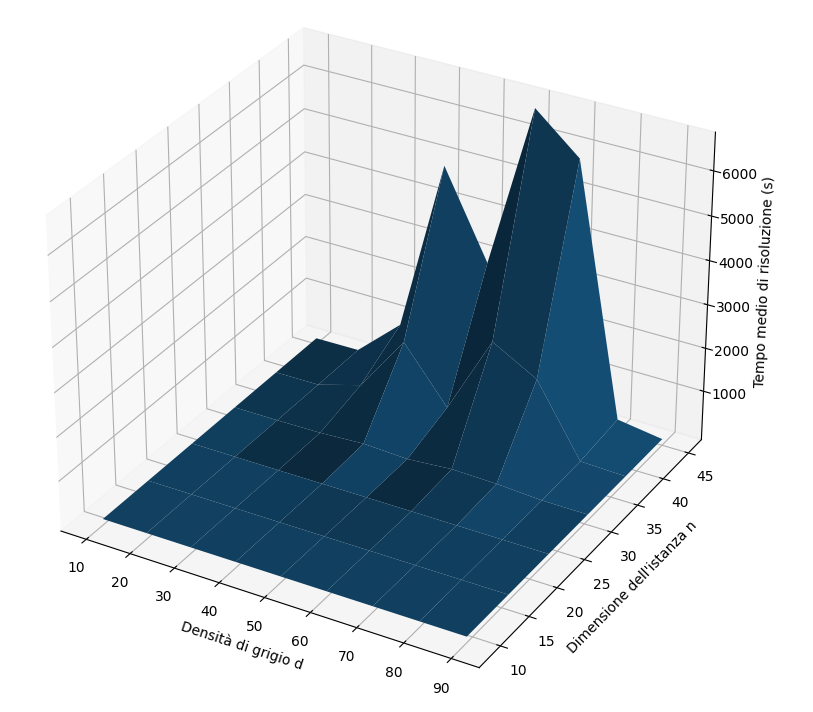
\includegraphics[scale=0.4]{images/resolution_times.png}
    \caption{Grafico dei tempi di risoluzione delle istanze Tai*c}
    \label{fig:times}
\end{figure}

\newpage
\section{Soluzioni trovate}